\documentclass[11pt,a4j, titlepage]{jarticle} %titlepageで表紙のページ番号をなくす
\usepackage[dvipdfmx,dvips]{graphicx}
\usepackage{otf}
\usepackage{amsmath,amssymb}
\usepackage{ascmac,here,txfonts}
\usepackage{listings,jlisting}
\usepackage{color}
\usepackage{epsfig}
\usepackage{fancybox}
\usepackage{epstopdf}
\usepackage{bm}
\usepackage{cases}
\usepackage{comment}
\usepackage{setspace}
\usepackage{uft}
\usepackage{subcaption}
\usepackage{array}
%%% jdummy.def
%
\DeclareRelationFont{JY1}{mc}{it}{}{OT1}{cmr}{it}{}
\DeclareRelationFont{JT1}{mc}{it}{}{OT1}{cmr}{it}{}
\DeclareFontShape{JY1}{mc}{m}{it}{<5> <6> <7> <8> <9> <10> sgen*min
    <10.95><12><14.4><17.28><20.74><24.88> min10
    <-> min10}{}
\DeclareFontShape{JT1}{mc}{m}{it}{<5> <6> <7> <8> <9> <10> sgen*tmin
    <10.95><12><14.4><17.28><20.74><24.88> tmin10
    <-> tmin10}{}
\DeclareRelationFont{JY1}{mc}{sl}{}{OT1}{cmr}{sl}{}
\DeclareRelationFont{JT1}{mc}{sl}{}{OT1}{cmr}{sl}{}
\DeclareFontShape{JY1}{mc}{m}{sl}{<5> <6> <7> <8> <9> <10> sgen*min
    <10.95><12><14.4><17.28><20.74><24.88> min10
    <-> min10}{}
\DeclareFontShape{JT1}{mc}{m}{sl}{<5> <6> <7> <8> <9> <10> sgen*tmin
    <10.95><12><14.4><17.28><20.74><24.88> tmin10
    <-> tmin10}{}
\DeclareRelationFont{JY1}{mc}{sc}{}{OT1}{cmr}{sc}{}
\DeclareRelationFont{JT1}{mc}{sc}{}{OT1}{cmr}{sc}{}
\DeclareFontShape{JY1}{mc}{m}{sc}{<5> <6> <7> <8> <9> <10> sgen*min
    <10.95><12><14.4><17.28><20.74><24.88> min10
    <-> min10}{}
\DeclareFontShape{JT1}{mc}{m}{sc}{<5> <6> <7> <8> <9> <10> sgen*tmin
    <10.95><12><14.4><17.28><20.74><24.88> tmin10
    <-> tmin10}{}
\DeclareRelationFont{JY1}{gt}{it}{}{OT1}{cmbx}{it}{}
\DeclareRelationFont{JT1}{gt}{it}{}{OT1}{cmbx}{it}{}
\DeclareFontShape{JY1}{mc}{bx}{it}{<5> <6> <7> <8> <9> <10> sgen*goth
    <10.95><12><14.4><17.28><20.74><24.88> goth10
    <-> goth10}{}
\DeclareFontShape{JT1}{mc}{bx}{it}{<5> <6> <7> <8> <9> <10> sgen*tgoth
    <10.95><12><14.4><17.28><20.74><24.88> tgoth10
    <-> tgoth10}{}
\DeclareRelationFont{JY1}{gt}{sl}{}{OT1}{cmbx}{sl}{}
\DeclareRelationFont{JT1}{gt}{sl}{}{OT1}{cmbx}{sl}{}
\DeclareFontShape{JY1}{mc}{bx}{sl}{<5> <6> <7> <8> <9> <10> sgen*goth
    <10.95><12><14.4><17.28><20.74><24.88> goth10
    <-> goth10}{}
\DeclareFontShape{JT1}{mc}{bx}{sl}{<5> <6> <7> <8> <9> <10> sgen*tgoth
    <10.95><12><14.4><17.28><20.74><24.88> tgoth10
    <-> tgoth10}{}
\DeclareRelationFont{JY1}{gt}{sc}{}{OT1}{cmbx}{sc}{}
\DeclareRelationFont{JT1}{gt}{sc}{}{OT1}{cmbx}{sc}{}
\DeclareFontShape{JY1}{mc}{bx}{sc}{<5> <6> <7> <8> <9> <10> sgen*goth
    <10.95><12><14.4><17.28><20.74><24.88> goth10
    <-> goth10}{}
\DeclareFontShape{JT1}{mc}{bx}{sc}{<5> <6> <7> <8> <9> <10> sgen*tgoth
    <10.95><12><14.4><17.28><20.74><24.88> tgoth10
    <-> tgoth10}{}
\DeclareRelationFont{JY1}{gt}{it}{}{OT1}{cmr}{it}{}
\DeclareRelationFont{JT1}{gt}{it}{}{OT1}{cmr}{it}{}
\DeclareFontShape{JY1}{gt}{m}{it}{<5> <6> <7> <8> <9> <10> sgen*goth
    <10.95><12><14.4><17.28><20.74><24.88> goth10
    <-> goth10}{}
\DeclareFontShape{JT1}{gt}{m}{it}{<5> <6> <7> <8> <9> <10> sgen*tgoth
    <10.95><12><14.4><17.28><20.74><24.88> tgoth10
    <-> tgoth10}{}
\DeclareFontShape{JY1}{mc}{m}{sc}{<5> <6> <7> <8> <9> <10> sgen*min
    <10.95><12><14.4><17.28><20.74><24.88> min10
    <-> min10}{}
\DeclareFontShape{JT1}{mc}{m}{sc}{<5> <6> <7> <8> <9> <10> sgen*tmin
    <10.95><12><14.4><17.28><20.74><24.88> tmin10
    <-> tmin10}{}
\endinput
%%%% end of jdummy.def


\definecolor{dkgreen}{rgb}{0,0.6,0} 
\definecolor{gray}{rgb}{0.5,0.5,0.5}
\definecolor{mauve}{rgb}{0.58,0,0.82}
\setlength{\oddsidemargin}{0mm}
\setlength{\textwidth}{170mm} 
\setlength{\topmargin}{-5mm}
\setlength{\textheight}{240mm}
\setlength{\columnsep}{8mm}
\setlength{\oddsidemargin}{-1.04cm}

\begin{document}

%タイトル
\begin{titlepage}
	\begin{center}
		\vspace{8ex}
		{\Large \bf 平成27年度卒業論文}
		\vspace{3ex}\\
		\rule{\hsize}{2mm}
		\vspace{1mm}\\ 
		{\LARGE \bf FingCV: スマートフォンの内蔵カメラを用いたジェスチャによる簡易操作法の提案・実装・評価} 
		\vspace{6mm}\\ 
		\rule{\hsize}{2mm} 
		\vspace{2.5cm} \\ 
		{\Large 電気通信大学 情報理工学部 \\ 
		情報・通信工学科 コンピュータサイエンスコース} 
		\vspace{2ex} \\ 
		\renewcommand{\thefootnote}{\fnsymbol{footnote}} 
		{\Large 赤 池 H I\footnote{Human Interface} 研 究 室} 
		\vspace{3ex} \\ 
		{\Large 指導教員 : 赤 池 \ 英 夫 ({\em Akaike Hideo})} 
		\vspace{3ex} \\
		{\Large 学籍番号 : 1211019 \ / \ 猪 膝 \ 孝 之 ({\em Inohiza Takayuki})} 
		\vspace{5ex} \\ 
		{\Large 提出日 : 平成 28 年 2 月 1 日 ( 月 )} 
		\vspace{-5ex} \\ 
		\begin{verbatim} 
		\end{verbatim} 
	\end{center} 
\end{titlepage}

%概要
\begin{abstract}
	\ \ \ 本研究では、スマートフォンの内蔵カメラを用いて指のジェスチャを認識して操作をする方法について提案、実装し、有用性について評価した。

	近年スマートフォンが普及してきており、タッチ操作が可能になった事によって、ユーザーは従来の携帯電話よりも直感的な操作を行う事が出来るようになった。加えて、スマートフォンは以前よりも画面表示領域が大きくなっている。しかし、ユーザーがコンテンツを視認する際に手や指が邪魔になり、スマートフォンの表示領域の広さを最大限生かせなくなる。

	そこで本研究はスマートフォンの内蔵カメラを利用して指のジェスチャを認識することによって、表示領域の広さを生かすような操作方法を提案し、実装した。また、独自のテスト用ページを作成し、被験者のブラウジング実験により有用性について評価した。

	実験結果よりFingCVのほうがセッション数を増やせば増やすほどタスク完了時間が低下することがわかった。操作に慣れない人も多く、スクロールやズームの精度がそこまで良くなかったため、被験者8人中良いと思った人が1人、普通と思った人が4人、悪いと思った人が3人とFingCVの総合的な評価としてはあまり良くなかった。個人差もかなりあったように見られた。画面の表示領域を最大限生かすという点は、FingCVの場合スクロールやズームをしている際、画面全体の把握がしやすかったどうかという設問で、とても把握しやすいと思った人が2人、把握しやすいと思った人が3人と回答しており、改善されたという意見が多かったことがわかった。しかし、カメラのプレビュー画面に集中しすぎて画面全体が見づらくなってしまうという問題点も挙がった。

\end{abstract}

%目次
\tableofcontents
\newpage
\listoffigures
\newpage
\listoftables
\newpage
\section{はじめに}
\subsection{研究背景}
近年、従来の携帯電話の代わりにスマートフォンの急速な普及が見られる。スマートフォンは、従来の携帯電話に比べて画面の表示領域が広いことに加えて、タッチして操作する事が可能となっている点が特徴である。

タッチ操作が可能になった事によって、ユーザーは従来の携帯電話よりも直観的な操作を行う事ができるようになった。しかし、コンテンツを視認する際にタッチ操作では手や指が邪魔になり、スマートフォンの表示領域の広さを最大限生かせなくなる。

画面の表示領域を最大限生かすために端末の背面に背面タッチが可能になるようなハードウェアを取り付けることによって背面からの端末の操作にする研究[1][2]が行われてきた。しかし、欠点として可搬性が制限されてしまったり、独自のハードウェアとして専用の部品を取り付ける必要がある。

他には内蔵カメラを用いて指を認識しジェスチャを検出することによって端末を操作を可能にする研究[3][4]が行われてきた。しかし、欠点としてスワイプ操作しかできないので機能性が欠ける。

そこで、独自のハードウェアを装着することなく、機能性を向上させることができないかと考え、本研究の立案に至った。
\subsection{研究目的}
本研究は、どの端末でも付属している内蔵カメラを用いて画面の表示領域を狭める事なく、スマートフォンを操作するような手法を提案、実装を行った。その後、評価実験を行い、有用性について評価を行った。

\newpage
\section{関連研究}
\subsection{はじめに}
この章では、画面の表示領域を最大限生かすことを目的とした既存の研究についてそれぞれ特徴や問題点を述べる。

\subsection{背面から端末を操作}
Wigdorら[1]の研究では図\ref{wigdor}のようにディスプレイの背面にタッチパッドとカメラを装着し、背面からの操作を可能にしている。しかし、背面にカメラを取り付けるために可搬性が制限されてしまうという問題がある。

小林ら[2]の研究では図\ref{kobayashi}のように端末の背面にタッチパネルを取り付けて画面領域を狭める事なく操作をする方法を可能としている。しかし、独自のハードウェアを装着する必要があることが問題として考えられる。

\begin{figure}[H]
	\centering
	\begin{subfigure}{0.4\columnwidth}
		\centering
		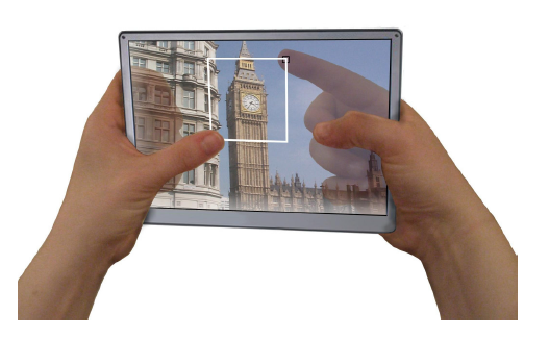
\includegraphics[width=\columnwidth]{lucid.eps}
		\caption{Wigdorらの研究}
		\label{wigdor}
	\end{subfigure}
	\begin{subfigure}{0.4\columnwidth}
		\centering
		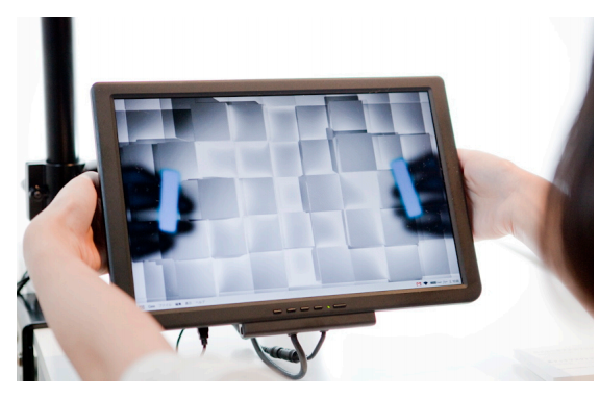
\includegraphics[width=\columnwidth]{uratouch.eps}
		\caption{小林らの研究}
		\label{kobayashi}
	\end{subfigure}
	\caption{背面から端末を操作}
	\label{fig:f1}
\end{figure}


\subsection{内蔵カメラを用いて端末を操作}
竹田ら[3]の研究では図\ref{fig:1a}のように端末の背面カメラで指を認識し上下左右の4方向のジェスチャを検出することによって操作する手法を実現した。また、それを改良した研究[4]では図\ref{fig:1b}より斜め移動が加わり、より自由度の高いジェスチャの検出することが可能となっている。しかし、この研究は検討段階であり、実際に実装されたわけではない。加えて、使用できるジェスチャの数が限定されてしまい、スワイプ操作しかできないので機能性が欠けることが考えられる。

\begin{figure}[H]
	\centering
	\begin{subfigure}{0.4\columnwidth}
		\centering
		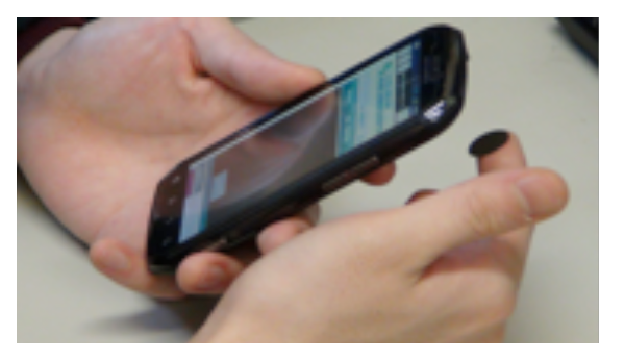
\includegraphics[width=\columnwidth,height=4cm]{cameragesture1.eps}
		\caption{上下左右の4方向のジェスチャを検出}
		\label{fig:1a}
	\end{subfigure}
	\begin{subfigure}{0.4\columnwidth}
		\centering
		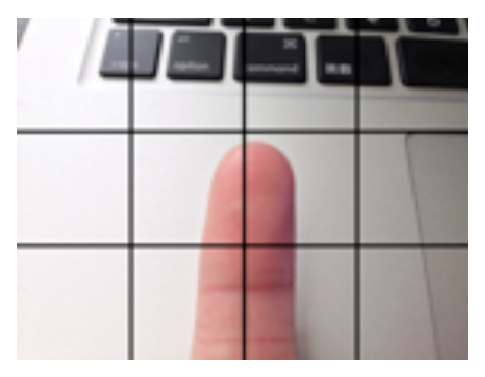
\includegraphics[width=\columnwidth,height=4cm]{cameragesture2.eps}
		\caption{斜め移動のジェスチャの検出が可能}
		\label{fig:1b}
	\end{subfigure}
	\caption{内蔵カメラを用いて端末を操作}
	\label{fig:f2}
\end{figure}

\subsection{おわりに}
本章では、画面の表示領域を最大限生かすことを目的とした既存の研究について述べた。次章では、本研究で作成したシステム、FingCVの概要について述べる。

\newpage
\section{本システム(FingCV)の概要}
\subsection{はじめに}
この章では、本研究で作成したシステム、FingCVについて詳しく述べる。最初に、システムの主な仕様、操作方法について説明をし、その次に実装したそれぞれの機能について述べる。
\subsection{主な仕様、操作方法}
ここではブラウザ利用時を想定する。右利きの場合、図\ref{fig:f3}のように左手でスマートフォンを持ち、右手の指を背面カメラで読み取って、指の動きを認識することによってジェスチャを検出する。

\begin{figure}[H]
	\centering
	\includegraphics[width=5cm,height=4cm]{teyubi.eps}
	\caption{操作方法}
	\label{fig:f3}
\end{figure}

図\ref{fig:f4}のような画面の端の特定の位置を押したままにすることによって操作モードが切り替わるようにする。操作モードは以下の3つである。
\begin{itemize}
	\item スワイプ操作
	\item ピンチイン、ピンチアウト操作
	\item 閲覧履歴の移動操作
\end{itemize}

\begin{figure}[H]
	\centering
	\centering
	\includegraphics[width=6cm,height=8cm]{hasi.eps}
	\caption{画面の端の特定の位置}
	\label{fig:f4}
\end{figure}

図\ref{fig:f5}のように右利き用には画面右下でカメラのプレビューを見ることができるようになっており、指がカメラに写っているかどうかを確認することができる。

\begin{figure}[H]
	\centering
	\includegraphics[width=6cm,height=8cm]{gamen.eps}
	\caption{動作時の画面}
	\label{fig:f5}
\end{figure}

図\ref{fig:f6}はカメラのプレビュー画面である。この画面には赤い丸い円が描画されており、初期位置としてこの円の中に指先を写すようにする。

\begin{figure}[H]
	\centering
	\includegraphics[width=6cm,height=8cm]{shokiichi.eps}
	\caption{初期位置}
	\label{fig:f6}
\end{figure}

\subsection{スワイプ操作}
右利き用の場合、図\ref{fig:f7}のように画面の左下の位置を指で押したままにしている時、スワイプ操作モードに移行する(左利き用は画面の右下の位置)。スワイプとは画面に触れた状態で指を滑らせる動作のことである。

\begin{figure}[H]
	\centering
	\begin{subfigure}{0.4\columnwidth}
		\centering
		\includegraphics[width=\columnwidth,height=8cm]{hasi.eps}
		\caption{画面の端(左下)}
		\label{fig:hasi1}
	\end{subfigure}
	\begin{subfigure}{0.4\columnwidth}
		\centering
		\includegraphics[width=\columnwidth,height=8cm]{hidarisita.eps}
		\caption{左下の位置を長押し}
		\label{fig:chuousita}
	\end{subfigure}
	\caption{画面の左下の位置}
	\label{fig:f7}
\end{figure}

まず、初期位置である赤い丸い円の中に指先を写すようにする。円の中から外に向かって指先を移動させ、指先が円の外に出た際にジェスチャを検出する。図\ref{fig:f8}のように8方向の移動が可能である。タッチ操作のスワイプと同様の方向に動かすようにする。例えば、指先を円の中から左方向に移動させると画面は右方向にスクロールをし、円の中から下方向に移動させると画面は上方向にスクロールする。

\begin{figure}[H]
	\centering
	\includegraphics[width=6cm,height=8cm]{swipe.eps}
	\caption{スワイプ操作}
	\label{fig:f8}
\end{figure}

\subsection{ピンチイン、ピンチアウト操作}
図\ref{fig:f9}のように画面の中央下の位置を指で押したままにしている時、ピンチイン、ピンチアウト操作モードに移行する。ピンチインとは二本の指を画面上にのせてその間隔を縮める動作のことで、反対にピンチアウトはその間隔を広げる動作のことである。

\begin{figure}[H]
	\centering
	\begin{subfigure}{0.4\columnwidth}
		\centering
		\includegraphics[width=\columnwidth,height=8cm]{hasi.eps}
		\caption{画面の端(中央下)}
		\label{fig:hasi2}
	\end{subfigure}
	\begin{subfigure}{0.4\columnwidth}
		\centering
		\includegraphics[width=\columnwidth,height=8cm]{chuousita.eps}
		\caption{中央下の位置を長押し}
		\label{fig:chuousita}
	\end{subfigure}
	\caption{画面の中央下の位置}
	\label{fig:f9}
\end{figure}

まず、初期位置である赤い丸い円の中に指先を写すようにする。図\ref{fig:pinchin}のように指先を円の中から上方向に移動させるとピンチイン(縮小)操作をし、図\ref{fig:pinchout}のように円の中から下方向に移動させるとピンチアウト(拡大)操作をする。

\begin{figure}[H]
	\centering
	\begin{subfigure}{0.4\columnwidth}
		\centering
		\includegraphics[width=\columnwidth,height=8cm]{pinchin.eps}
		\caption{ピンチイン(縮小)操作}
		\label{fig:pinchin}
	\end{subfigure}
	\begin{subfigure}{0.4\columnwidth}
		\centering
		\includegraphics[width=\columnwidth,height=8cm]{pinchout.eps}
		\caption{ピンチアウト(拡大)操作}
		\label{fig:pinchout}
	\end{subfigure}
	\caption{ピンチイン、ピンチアウト操作}
	\label{fig:f10}
\end{figure}

\subsection{閲覧履歴の移動操作}
閲覧履歴とはブラウザの履歴のことであり、履歴がある場合は進んだり戻ったりすることができる。右利き用の場合、図\ref{fig:f11}のように画面の右下の位置を指で押し続けている時、閲覧履歴の移動操作モードに移行する(左利き用は画面の左下の位置)。

\begin{figure}[H]
	\centering
	\begin{subfigure}{0.4\columnwidth}
		\centering
		\includegraphics[width=\columnwidth,height=8cm]{hasi.eps}
		\caption{画面の端(右下)}
		\label{fig:hasi3}
	\end{subfigure}
	\begin{subfigure}{0.4\columnwidth}
		\centering
		\includegraphics[width=\columnwidth,height=8cm]{migisita.eps}
		\caption{右下の位置を長押し}
		\label{fig:chuousita}
	\end{subfigure}
	\caption{画面の右下の位置}
	\label{fig:f11}
\end{figure}

まず、初期位置で赤い丸い円の中に指先を写すようにする。図\ref{fig:goforward}のように指先を円の中から右方向に移動させると閲覧履歴を一つ進むことができ、図\ref{fig:goback}のように円の中から左方向に移動させると閲覧履歴を一つ戻ることができる。履歴がない場合はページは変化しない。

\begin{figure}[H]
	\centering
	\begin{subfigure}{0.4\columnwidth}
		\centering
		\includegraphics[width=\columnwidth,height=8cm]{goforward.eps}
		\caption{閲覧履歴を一つ進める操作}
		\label{fig:goforward}
	\end{subfigure}
	\begin{subfigure}{0.4\columnwidth}
		\centering
		\includegraphics[width=\columnwidth,height=8cm]{goback.eps}
		\caption{閲覧履歴を一つ戻る操作}
		\label{fig:goback}
	\end{subfigure}
	\caption{閲覧履歴の移動操作}
	\label{fig:f12}
\end{figure}

\subsection{おわりに}
本章では本研究で作成したシステム、FingCVについての主な仕様、操作方法について説明をし、その後に実装したそれぞれの機能について述べた。次章では、FingCVの実装環境や実装方法について詳しく述べる。

\newpage
\section{実装}
\subsection{はじめに}
この章では最初に本研究で作成したシステム、FingCVについての実装環境について説明をする。その次に指認識の方法について詳しく説明した後にブラウザの操作処理について詳しく述べる。

\subsection{実装環境}
システムにはプログラミング言語としてJavaを使い、Android上に作成した。Android端末はGALAXY S3(SC-06D)を使用した。指認識には画像処理ライブラリのOpenCV for Androidを使用し、Webページの表示にはWebViewを使用した。

\subsection{指認識}
ここではブラウザの操作をするため作成した指の検出の概要と流れを述べる。指の検出は画像処理によって行い、流れは図\ref{fig:f13}のようになっている。既存の研究[5]の手法を参考にして指認識の手法を考案した。また、本研究では画像処理による指先の検出を実現するためにOpenCV for Androidを使用した。

\begin{figure}[H]
	\centering
	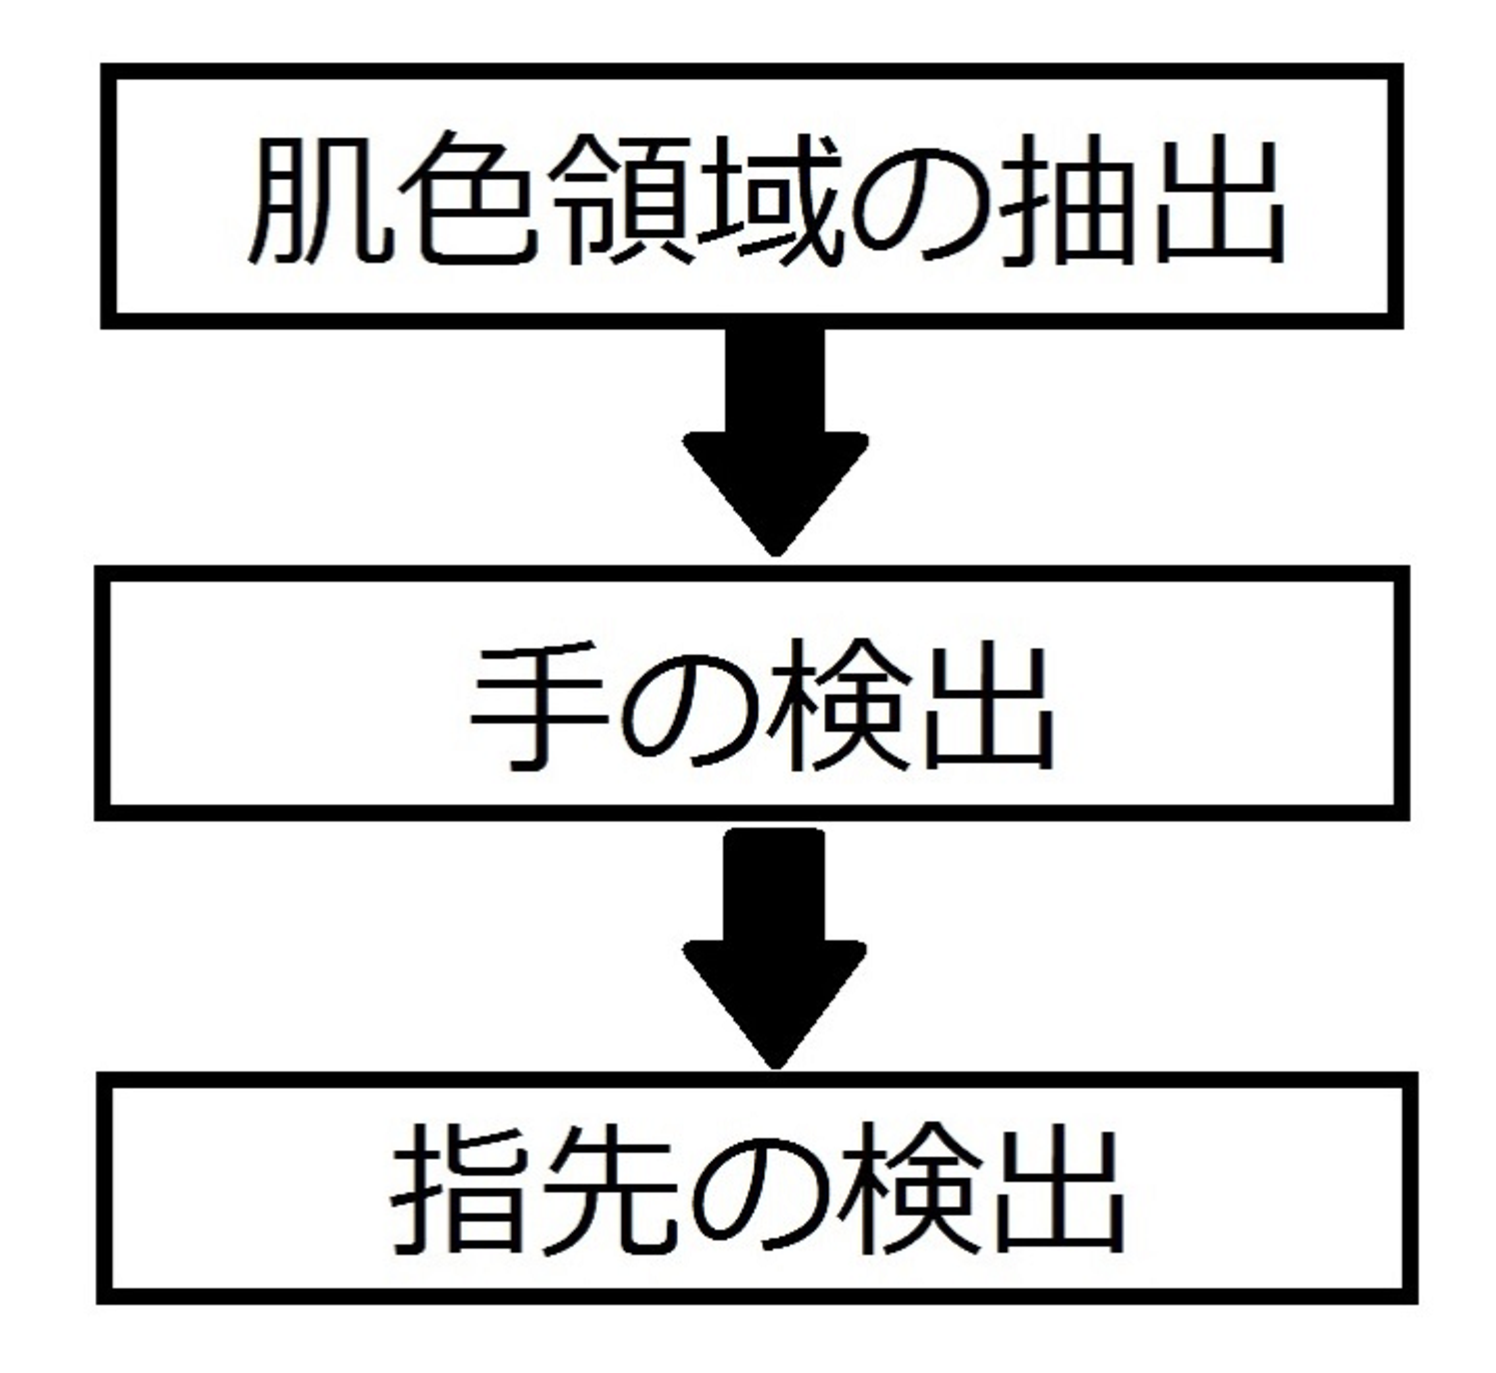
\includegraphics[width=6cm,height=6cm]{yubisakinagare.eps}
	\caption{指先の検出}
	\label{fig:f13}
\end{figure}

指先の検出には、最初にカメラの画面内に表示される肌色領域を抽出する。次に肌色領域の最大のところを手と判断し、ラベリングをし輪郭線を取得する。その後に指先を検出する。それぞれの詳細については以降に述べる。

\subsubsection{肌色領域の抽出}
指先を検出するために、まずカメラから入力された画像から肌色にあたる領域を抽出する。一般的な肌色領域の抽出方法としてはカメラによって入力されたRGB表色系の画像を他の画像に変換した後、画像の2値化という作業を行う。画像の2値化とは、任意の方法で検出したい色の閾値を決め、その閾値を元に画像を二色に分別する作業である。2値化の例を図\ref{fig:f14}に示す。肌色の2値化としては、肌色にあたる色の閾値を決め、その閾値から2値化をし、肌色であるか否かを判断する。また、RGB表色系の画像を用いない理由は、RGB表色系ではR・G・Bのような単色の検出率は非常に高いが、肌色のような混合色を抽出する場合、RGB表色系では混合色は広範囲に分布するため、閾値を決める方法で肌色領域を抽出する事は誤検出が非常に多くなるからである。RGB表色系を変換する表色系にHSV表色系を用いた。HSV表色系とは、1978年にアルヴィ・レイ・スミス(Alvy Ray Smith)によって考案された表色系であり、色相(Hue)、彩度(Saturation・Chroma)、明度(Brightness・Lightness・Value)の三つの成分からなる表色系であり、これはRGB色空間の非線形空間である。HSV表色系を用いる理由としては肌色の分布する範囲が狭いという特徴があるからである。肌色を抽出するためのHSV表色系でのH・S・Vのそれぞれの閾値を以下に示す。

\begin{itemize}
	\item Hue: 0<H<25
	\item Saturation: 58<S<173
	\item Value: 88<V<229
\end{itemize}

\begin{figure}[H]
	\centering
	\begin{subfigure}{0.4\columnwidth}
		\centering
		\includegraphics[width=\columnwidth,height=8cm]{nichikamae.eps}
		\caption{2値化処理前}
		\label{fig:nichikamae}
	\end{subfigure}
	\begin{subfigure}{0.4\columnwidth}
		\centering
		\includegraphics[width=\columnwidth,height=8cm]{nichikago.eps}
		\caption{2値化処理後}
		\label{fig:nichikago}
	\end{subfigure}
	\caption{2値化の例}
	\label{fig:f14}
\end{figure}

\subsubsection{手の検出}
次に目的の指先を検出するために手を検出する。手を検出する際に留意点としては、手以外で肌色に近い色の物体が存在する可能性を考慮しなければならない。本研究のシステムではカメラから入力される画像中の最大面積の肌色の物体を手とした。処理の軽減のため距離変換画像を用いた。距離変換とは二値画像の中にいくつか存在する物体の画素値(画素の明るさを表す数値)を、その物体の任意の画素から背景画素(画素値が0)までの最短距離を求め、画素値を置き換える処理である。変換して得られた画像を距離変換画像という。図\ref{fig:f15}に距離変換処理の例をあげる。

\begin{figure}[H]
	\centering
	\begin{subfigure}{0.4\columnwidth}
		\centering
		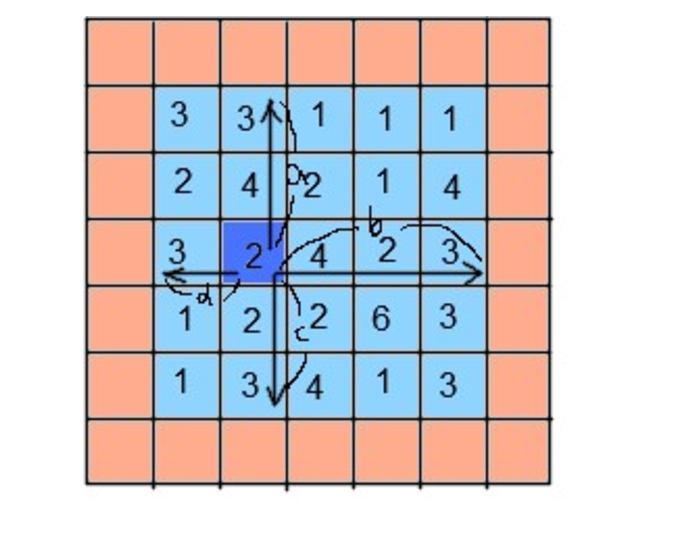
\includegraphics[width=\columnwidth,height=5cm]{henkanmae.eps}
		\caption{距離変換前}
		\label{fig:henkanmae}
	\end{subfigure}
	\begin{subfigure}{0.4\columnwidth}
		\centering
		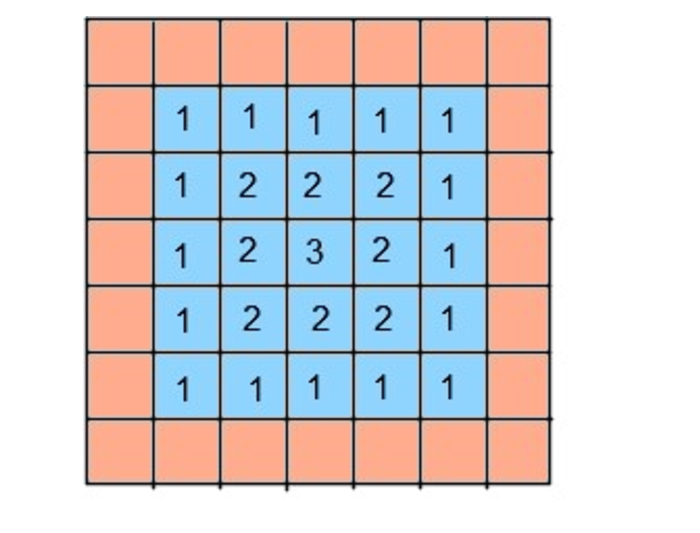
\includegraphics[width=\columnwidth,height=5cm]{henkango.eps}
		\caption{距離変換後}
		\label{fig:henkango}
	\end{subfigure}
	\caption{距離変換処理}
	\label{fig:f15}
\end{figure}

上の方法を用いて手を検出する方法をまとめると、手はカメラからの画像中最大の面積を持つ肌色領域としているので、背景から最も遠い画素の画素値が画像中最大になる事になる。つまり、距離変換画像中の最大の画素値を持つ肌色領域が手という事になる。

図\ref{fig:f16}が手を検出した例である。

\begin{figure}[H]
	\centering
	\includegraphics[width=6cm,height=6cm]{tekenshutu.eps}
	\caption{手の検出}
	\label{fig:f16}
\end{figure}

\subsubsection{指先の検出}
次に指先の検出方法について述べる。まず、最初に図\ref{fig:f21}のように先ほど抽出された肌色領域の重心を求めて、その重心より上を指と判断するようにする。

\begin{figure}[H]
	\centering
	\includegraphics[width=6cm,height=6cm]{jusin.eps}
	\caption{肌色領域の重心}
	\label{fig:f21}
\end{figure}

次に指という形状を生かして輪郭の凹凸の有無と凹凸の方向から判定を行う。先ほど抽出された肌色領域の輪郭の輪郭点を一定の間隔をあけ3点$P_1,P_2,P_3$で、始まりから終わりまで沿うようにして調べていく。調べる内容は画像中の座標、x、y座標であり、この3点$P_1,P_2,P_3$の座標情報から$P_2$を原点とし、図\ref{fig:f17}のようになす角度θを計算する。なす角度θが式\ref{eq:eq1}の際、その3点から作られる形状は凹凸の形状をしている判断する。なす角度の計算方法は$P_2$を原点とした$P_1,P_2,P_3$の内積の計算式\ref{eq:eq2}から算出する。

\begin{figure}[H]
	\centering
	\includegraphics[width=6cm,height=6cm]{yubisaki1.eps}
	\caption{内積によるなす角度}
	\label{fig:f17}
\end{figure}

\begin{eqnarray}
0°<&θ&<60° \label{eq:eq1} \\
P_1&=&(P_{1x}, P_{1y}) \\
P_2&=&(P_{2x}, P_{2y}) \\
P_3&=&(P_{3x}, P_{3y}) \\
C_1&=&(C_{1x}, C_{1y}) \\
C_{1x}&=&P_{1x}-P_{2x} \\
C_{1y}&=&P_{1y}-P_{2y} \\
C_2&=&(C_{2x}, C_{2y}) \\
C_{2x}&=&P_{3x}-P_{2x} \\
C_{2y}&=&P_{3y}P_{2y} \\
P_1P_2&=&C_1 \\
P_1P_2&=&C_2 \\
|P_1P_2|&=&|C_1| \\
|P_3P_2|&=&|C_2| \\
|C_1|&=&\sqrt{|C_{1x}|^2+|C_{2y}|^2} \\
|C_2|&=&\sqrt{|C_{2x}|^2+|C_{2y}|^2} \\
C_1・C_2&=&C_{1x}×C_{2x}+C_{1y}×C_{2y} \\
cos{θ}&=&\frac{C_1・C_2}{|C_1||C_2|} \label{eq:eq2}
\end{eqnarray}

次に凹凸の方向の判定を行う。凹凸の方向の判定には$P_2$を原点とした$P_1, P_2, P_3$の外積の式から算出される$sin{θ}$を使用した。本研究では$sin{θ}$が式\ref{eq:eq3}の時に凸と判定し、式\ref{eq:eq4}の時に凹と判定した。外積の計算には式\ref{eq:eq5}を使用した。

\begin{eqnarray}
0°<&θ&<90° \label{eq:eq3} \\
-90°<&θ&<0° \label{eq:eq4} \\
C_1×C_2&=&C_{1x}×C_{2y}-C_{2x}×C_{1y} \\
sin{θ}&=&\frac{C_1×C_2}{|C_1||C_2|} \label{eq:eq5}
\end{eqnarray}

次に人間の指は特殊な姿勢を除いては、基本的に上を向いているので凸の方向を向いている3点$P_1, P_2, P_3$を指と判定した。ここで先ほどの指先の検出の判定をまとめると内積から得られるなす角度θが式\ref{eq:eq1}の場合、かつ、外積から得られるなす角度が式\ref{eq:eq3}の場合、その3点は指だと判定している。ここまでの処理で指の判断は可能になったが、指と判断される3点は輪郭点の調査を手の輪郭点に対して全てに行う事から、図\ref{fig:f18}のように1つの指に対して多数存在する事になる。

\begin{figure}[H]
	\centering
	\includegraphics[width=6cm,height=6cm]{fukusukenshutu.eps}
	\caption{指と判断された多数の点}
	\label{fig:f18}
\end{figure}

次に先ほど多数検出された点の中で、ある2つの点が近い距離にある場合、それらを1つにする処理をする。図\ref{fig:f19}のようにそれぞれの点のx,y座標を足して2で割って1つにする処理をする。

\begin{figure}[H]
	\centering
	\begin{subfigure}{0.4\columnwidth}
		\centering
		\includegraphics[width=\columnwidth,height=6cm]{futatu.eps}
		\caption{距離が近い2つの点}
		\label{fig:futatu}
	\end{subfigure}
	\begin{subfigure}{0.4\columnwidth}
		\centering
		\includegraphics[width=\columnwidth,height=6cm]{hitotu.eps}
		\caption{1つの点にする}
		\label{fig:hitotu}
	\end{subfigure}
	\caption{2つの点を1つの点にする処理}
	\label{fig:f19}
\end{figure}

同様に検出された多数の点が1つの点になるまで繰り返し処理をする。図\ref{fig:f20}のように残った最後の1点を指先と判断する。

\begin{figure}[H]
	\centering
	\includegraphics[width=6cm,height=6cm]{saigo.eps}
	\caption{残った最後の1点}
	\label{fig:f20}
\end{figure}

\subsection{ブラウザの操作処理}
ここではブラウザの操作処理について詳しく説明をする。Webページの表示にはWebViewを使用する。右利きの場合、左手の親指で画面の特定の位置を長押しすることによって操作モード切り替える。以降は、操作モードの切り替え、指先のジェスチャ検出の処理方法について述べる。

\begin{figure}[H]
	\centering
	\includegraphics[width=9cm,height=6cm]{mode.eps}
	\caption{ブラウザの操作処理の概要}
	\label{fig:f22}
\end{figure}

\subsubsection{操作モードの切替}
右利きの場合、左手の親指で画面の特定の位置を長押しすることによって操作モード切り替える。どこも押してない場合は初期モード(mode=0)となっている。画面のサイズは縦が1280で、横が720で、左上を原点とする。画面を押している場所の座標を(pointX, pointY)として保存する。その時、操作モードの切替処理は以下のようになる。

\begin{itemize}
	\item 0$\le$pointX$\le$240かつ1120$\le$pointY$\le$1280のとき、mode=1(スワイプ操作モード)
	\item 241$\le$pointX$\le$480かつ1120$\le$pointY$\le$1280のとき、mode=2(ピンチイン、ピンチアウト操作モード)
	\item 481$\le$pointX$\le$720かつ1120$\le$pointY$\le$1280のとき、mode=3(閲覧履歴の移動操作モード)
\end{itemize}


\subsubsection{指先のジェスチャ検出}
まず、図\ref{fig:f23}のようにカメラのプレビュー画面に初期位置として赤い丸い円を描画する。この赤い円の中に指先(黄色の円)を写すとその座標を(yubi1.x, yubi1.y)として保存する。

\begin{figure}[H]
	\centering
	\includegraphics[width=6cm,height=8cm]{shokiichi.eps}
	\caption{初期位置として赤い円を描写}
	\label{fig:f23}
\end{figure}

指先が赤い円の外で検出された場合、Timer、TimerTaskを利用する。Timerクラスのscheduleメソッドを使用し、指定した時間に指定したタスクが実行されるようにスケジュールをする。本システムの場合は指先が赤い円の外で検出されて0.5秒にタスクが実行されるようにスケジュールをする。

タスクの内容はまず指先の座標を(yubi2.x, yubi2.y)として保存する。そして、yubi1.xとyubi2.x、yubi1.yとyubi2.yのそれぞれの差を取って一定の大きさ以上だった場合、指先のジェスチャを検出するようにする。

まず、スワイプ操作について詳しく説明する。WebViewクラスのscrollByメソッドを使用する。8方向のジェスチャの処理については以下のようにする。Nは15とし、shokika()ではyubi2.x=yubi1.x、yubi2.y=yubi1.yという処理をしている。

\begin{lstlisting}[basicstyle=\ttfamily\footnotesize, frame=single]
if (yubi2.x - yubi1.x > N && yubi2.y - yubi1.y <= N && yubi1.y - yubi2.y <= N) {
	if (0 < webView.getScrollY()) {
	webView.scrollBy(0, -50); // 上方向のスクロール
	}
	shokika();
} else if (yubi1.x - yubi2.x > N && yubi2.y - yubi1.y <= N && yubi1.y - yubi2.y <= N) {
	if (webView.getScrollY() < webView.getContentHeight() * webView.getScale()) {
		webView.scrollBy(0, 50); // 下方向のスクロール
	}
	shokika();
} else if (yubi2.y - yubi1.y > N && yubi2.x - yubi1.x <= N && yubi1.x - yubi2.x <= N) {
	if (webView.getScrollX() < 600 * webView.getScale()) {
		webView.scrollBy(50, 0); // 右方向のスクロール
	}
	shokika();
} else if (yubi1.y - yubi2.y > N && yubi2.x - yubi1.x <= N && yubi1.x - yubi2.x <= N) {
	if (0 < webView.getScrollX()) {
		webView.scrollBy(-50, 0); // 左方向のスクロール
	}
	shokika();
} else if (yubi1.x - yubi2.x > N && yubi1.y - yubi2.y > N) {
	if (webView.getScrollY() < webView.getContentHeight() * webView.getScale()
			&& 0 < webView.getScrollX()) {
		webView.scrollBy(0, 50); // 左下
		webView.scrollBy(-50, 0);
	}
	shokika();
} else if (yubi1.x - yubi2.x > N && yubi2.y - yubi1.y > N) {
	if (webView.getScrollY() < webView.getContentHeight() * webView.getScale()
			&& webView.getScrollX() < 600 * webView.getScale()) {
		webView.scrollBy(0, 50); // 右下
		webView.scrollBy(50, 0);
	}
	shokika();
} else if (yubi2.x - yubi1.x > N && yubi1.y - yubi2.y > N) {
	if (0 < webView.getScrollY() && 0 < webView.getScrollX()) {
		webView.scrollBy(0, -50); // 左上
		webView.scrollBy(-50, 0);
	}
	shokika();
} else if (yubi2.x - yubi1.x > N && yubi2.y - yubi1.y > N) {
	if (0 < webView.getScrollY() && webView.getScrollX() < 600 * webView.getScale()) {
		webView.scrollBy(0, -50); // 右上
		webView.scrollBy(50, 0);
	}
	shokika();
}
\end{lstlisting}

次にズームイン、ズームアウト操作について詳しく説明する。WebViewクラスのzoomIn、zoomOutメソッドを使用する。それぞれの操作については以下のようにする。

\begin{lstlisting}[basicstyle=\ttfamily\footnotesize, frame=single]
if (yubi2.x - yubi1.x > 22) {
	webView.zoomIn(); // ズームイン
	shokika();
} else if (yubi1.x - yubi2.x > 22) {
	webView.zoomOut(); // ズームアウト
	shokika();
}
\end{lstlisting}

次に閲覧履歴の移動操作について詳しく説明する。WebViewクラスのgoForward、goBackメソッドを使用する。それぞれの操作について以下のようにする。

\begin{lstlisting}[basicstyle=\ttfamily\footnotesize, frame=single]
if (yubi1.y - yubi2.y > 25) {
	webView.goForward(); // 進む
	shokika();
} else if (yubi2.y - yubi1.y > 25) {
	webView.goBack(); // 戻る
	shokika();
}
\end{lstlisting}

\subsection{おわりに}
本章では本研究で作成したシステム、FingCVについての実装環境について説明をし、指認識、ブラウザの操作処理の方法について詳しく説明をした。次章では評価実験について述べる。

\newpage
\section{評価実験}
\subsection{はじめに}
この章では本研究で作成したシステム、FingCVについての評価実験を行う。最初に実験目的について述べ、その後に実験内容について詳しく説明をする。

\subsection{実験目的}
本実験により、FingCVを使用することによってスマートフォンの表示領域の広さを最大限生かすことができたかどうかについて評価をする。被験者には実験後、アンケートに回答してもらいFingCVの使用感についても評価をする。

\subsection{被験者情報}
8人の被験者に本実験を依頼した。被験者全員の詳細なデータは下の表にまとめる。

\begin{table}[H]
	\begin{center}
	\begin{tabular}{|c|c|c|c|c|c|} \hline
		被験者No. & 性別 & 年齢 & 利き手 \\ \hline \hline
		01 & 男 & 21 & 右利き \\
		02 & 男 & 23 & 右利き \\
		03 & 男 & 22 & 右利き \\
		04 & 男 & 22 & 右利き \\
		05 & 男 & 23 & 左利き \\
		06 & 男 & 24 & 右利き \\
		07 & 女 & 20 & 右利き \\
		08 & 男 & 24 & 右利き \\ \hline
	\end{tabular}
	\caption{被験者情報}
	\label{table1}
	\end{center}
\end{table}

表\ref{table1}より、被験者の男女比は7:1で、年齢の中央値は22.5歳であった。全員学生であり、普段からスマートフォンを利用している。

\subsection{実験内容}
被験者に本システムであるFingCVとタッチ操作の方法で、図\ref{fig:f24}のような作成した独自のページについて実験を行った。作成した独自のページにはjQueryのプラグイン[6][7]を使用している。被験者には路線図の中からある特定の駅を探すタスクをFingCVのほうで10回、タッチ操作の方法で10回それぞれ行った。路線図を開いた時、開始時間を測定するようにし、特定の駅が見つかり、その場所をタッチした時、終了時間を測定するようにし、終了時間から開始時間を引いたものをタスク完了時間として測定した。測定をする前に被験者には慣れるまでそれぞれの操作の練習をしてもらった。被験者No.が奇数の人には最初にFingCVのほうで10回タスクを行った後に、タッチ操作の方法で10回行ってもらい、偶数の人には最初にタッチ操作の方法で10回タスク行った後に、FingCVのほうで10回行ってもらった。それぞれの正解の駅はランダムであり、池袋や上野のような利用者が多くて明らかに認知度が高い駅や一度出た駅は出ないようにした。

\begin{figure}[H]
	\centering
	\begin{subfigure}{0.4\columnwidth}
		\centering
		\includegraphics[width=\columnwidth,height=8cm]{fingcvgamen.eps}
		\caption{FingCV}
		\label{fig:fingcvgamen}
	\end{subfigure}
	\begin{subfigure}{0.4\columnwidth}
		\centering
		\includegraphics[width=\columnwidth,height=8cm]{touchgamen.eps}
		\caption{タッチ操作}
		\label{fig:touchgamen}
	\end{subfigure}
	\caption{実験時の画面}
	\label{fig:f24}
\end{figure}

\subsection{アンケート内容}
実験後、被験者にはFingCVの使用感についてアンケートで回答してもらった。アンケートの内容は以下である。

\begin{itemize}
	\item スクロールの精度についてはどうでしたか?
	\item ズームの精度はどうでしたか?
	\item 疲労感はありましたか?
	\item タッチ操作の場合、スクロールやズームをしている際に画面全体を把握しやすかったですか?
	\item 本システムの場合、スクロールやズームをしている際に画面全体を把握しやすかったですか?
	\item タッチ操作と比べて本システムはどうでしたか?
	\item 総合的に見て本システムはどうでしたか?
	\item 何か追加してほしい機能等はありますか?
	\item 何か気づいたこと等あればご自由にどうぞ
\end{itemize}

\subsection{おわりに}
本章では本実験の目的、実験内容、アンケート内容について詳しく述べた。次章では実験で得られたタスク完了時間の結果やアンケート結果について詳しく述べる。

\newpage
\section{実験の結果と考察}
\subsection{はじめに}
この章では本実験の測定結果やアンケート結果について詳しく述べる。それぞれの考察についても述べる。

\begin{comment}
\subsection{練習のべき乗則}
両対数グラフ上にプロットしたグラフが直線になるような関係があるとき、これらはべき乗則に従うという。例えば、2倍上達するのに100回の練習が必要なのであれば、$2×2=4倍$上達するのに$100×100=10000回$の練習が必要だということになる。練習量と上達度はおよそべき乗則に従うが、練習しても上達しない「スランプ」の時期が結構ある。スランプの時期は練習しても上達しないばかりか、かえって下手になっていくこともある。スランプを脱出すると一気に上達が進み、大局的にはべき乗則の通り上達が進む。以下は練習のべき乗則の式である。

n回目の試行にかかる時間$T_n$はべき乗則に従う。

\begin{eqnarray}
T_n=T_1n^{-α}
\end{eqnarray}

あるいは、
\begin{eqnarray}
log{T_n}=log{T_1}-αlog{n}
\end{eqnarray}

ただし、
\begin{eqnarray}
α=0.2~0.6
\end{eqnarray}
\end{comment}

\subsection{測定結果}
被験者8人のFingCVのほうのタスク完了時間は以下のようになった。

\begin{figure}[H]
	\centering
	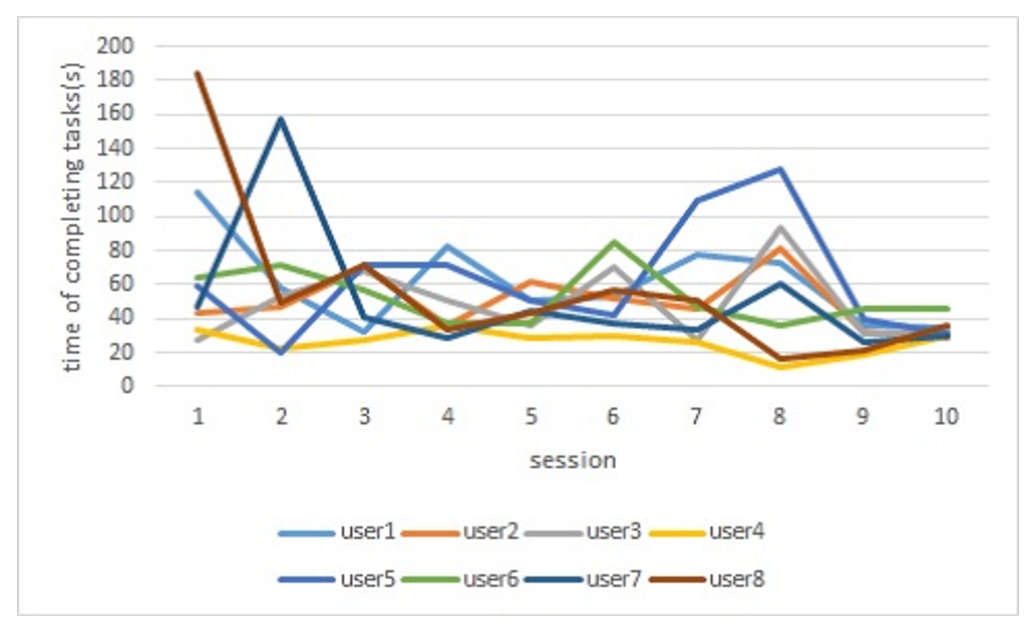
\includegraphics[width=10cm,height=7cm]{fingcvgraph.eps}
	\caption{FingCVで行った場合のタスク完了時間}
	\label{fig:f25}
\end{figure}

\begin{table}[H]
	\begin{center}
	\begin{tabular}{|c|c|c|c|c|c|c|c|c|c|c|} \hline
		user & 1 & 2 & 3 & 4 & 5 & 6 & 7 & 8 & 9 & 10\\ \hline \hline
		user 1 & 114.806 & 57.588 & 31.889 & 82.285 & 50.526 & 52.903 & 77.617 & 72.354 & 36.034 & 34.932\\
		user 2 &  43.218 & 47.418 & 70. 216 & 36.504 &61.229 & 51.901 & 45.806 & 81.283 & 31.669 & 27.949 \\
		user 3 &  26.824 & 53.46 & 68.106 & 50.858 & 36.452 & 70.822 & 27.045 & 93.365 & 30.571 & 31.772 \\
		user 4 &  33.812 & 22.704 & 27.016 & 35.812 & 28.923 & 30.349 &  26.721 & 11.236 & 18.7 & 29.546 \\
		user 5 &  59.211 & 20.43 & 71.151 & 71.697 & 50.737 & 42.415 & 108.932 & 127.294 & 39.299 & 30.519\\
		user 6 &  63.769 & 71.88 & 57.02 & 36.952 & 37.474 & 84.948 & 47.011 & 35.842 & 45.12 & 45.924\\
		user 7 &  47.308 & 156.765 & 40.68 & 28.174 & 44.001 & 37.012 & 33.869 & 59.931 & 25.506 & 29.636 \\
		user 8 &  183.779 & 49.882 & 71.324 & 33.603 & 43.751 & 57.333 & 50.102 & 16.657 & 21.341 & 35.358\\ \hline
	\end{tabular}
	\caption{ユーザーごとのタスク完了時間(FingCVの場合)}
	\label{table9}
	\end{center}
\end{table}

\begin{table}[H]
	\begin{center}
	\begin{tabular}{|c|c|c|c|} \hline
		user & 平均 & 平均(6~10) & 平均(9~10)\\ \hline \hline
		user 1 & 61.0934 & 54.768 & 35.483\\
		user 2 & 49.7703 & 47.7216 & 29.809\\
		user 3 & 48.9274 &  50.715 & 31.1715\\
		user 4 & 26.4819 & 23.3104 & 24.123\\
		user 5 & 62.1685 & 69.6918 & 34.909\\
		user 6 & 52.603 & 51.787 & 45.567\\
		user 7 & 50.2882 & 37.1908 & 27.571\\
		user 8 & 56.313 & 36.1582 & 28.3495\\ \hline
	\end{tabular}
	\caption{ユーザーごとのタスク完了時間の平均(FingCVの場合)}
	\label{table11}
	\end{center}
\end{table}

タッチ操作のほうのタスク完了時間は以下のようになった。

\begin{figure}[H]
	\centering
	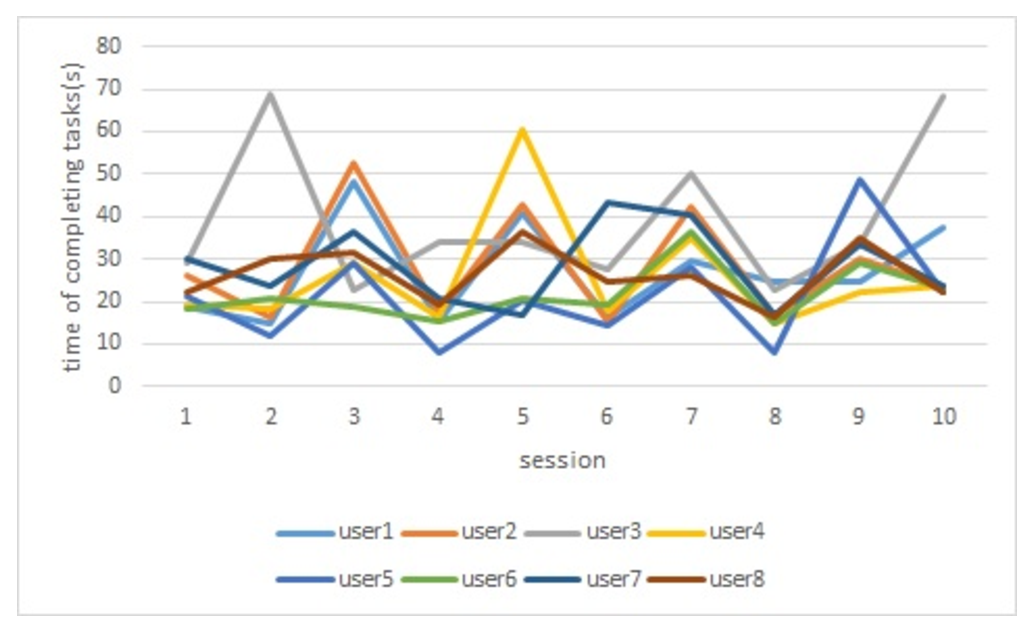
\includegraphics[width=10cm,height=7cm]{touchgraph.eps}
	\caption{タッチ操作で行った場合のタスク完了時間}
	\label{fig:f26}
\end{figure}

\begin{table}[H]
	\begin{center}
	\begin{tabular}{|c|c|c|c|c|c|c|c|c|c|c|} \hline
		user & 1 & 2 & 3 & 4 & 5 & 6 & 7 & 8 & 9 & 10\\ \hline \hline
		user 1 & 18.594 & 14.76 & 48.0895 & 15.471 & 40.895 & 16.112 & 29.361 & 24.825 & 24.568 & 37.239 \\
		user 2 &  26.341 & 16.304 & 52.806 & 17.455 & 42.814 & 15.387 & 42.525 & 16.75 & 30.207 & 23.626 \\
		user 3 &  29.064 & 68.713 & 22.504 & 33.809 & 33.809 & 27.666 & 50.134 & 22.696 & 33.6 & 68.144\\
		user 4 &  19.322 & 18.355 & 28.85 & 16.118 & 60.248 & 17.979 & 34.95 & 14.84 & 22.141 & 23.7\\
		user 5 &  21.124 & 11.808 & 28.853 & 8.113 & 20.159 & 14.152 & 28.341 & 8.213 & 48.636 & 22.272\\
		user 6 &  18.24 & 20.897 & 18.962 & 15.407 & 20.586 & 19.283 & 36.651 & 14.693 & 28.912 & 22.976\\
		user 7 &  30.199 & 23.566 & 36.409 & 20.787 & 16.745 & 43.175 & 40.157 & 16.58 & 33.42 & 23.878\\
		user 8 &  22.14 & 30.246 & 31.462 & 19.185 & 36.515 & 24.738 & 26.136 & 16.408 & 34.843 & 22.193\\ \hline
	\end{tabular}
	\caption{ユーザーごとのタスク完了時間(タッチ操作の場合)}
	\label{table10}
	\end{center}
\end{table}

\begin{table}[H]
	\begin{center}
	\begin{tabular}{|c|c|c|c|} \hline
		user & 平均 & 平均(6~10) & 平均(9~10)\\ \hline \hline
		user 1 & 26.99145 & 26.421 & 30.9035\\
		user 2 & 28.4215 & 25.699 & 26.9165\\
		user 3 & 39.0139 & 40.448 & 50.872\\
		user 4 & 25.6503 & 22.722 & 22.9205\\
		user 5 & 21.1671 & 24.3228 & 35.454\\
		user 6 & 21.6607 & 24.503 & 25.944\\
		user 7 & 28.4916 & 31.442 & 28.649\\
		user 8 & 26.3866 & 24.8636 & 28.518\\ \hline
	\end{tabular}
	\caption{ユーザーごとのタスク完了時間の平均(タッチ操作の場合)}
	\label{table12}
	\end{center}
\end{table}


\begin{comment}
FingCVのほうのタスク完了時間の低下予測は以下のようになった。

\begin{figure}[H]
	\centering
	\vspace{-50pt}
	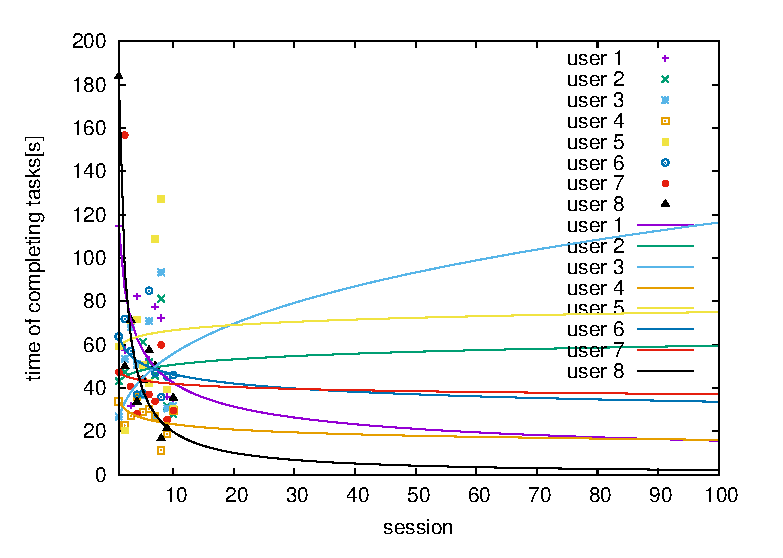
\includegraphics[width=12cm,height=8cm]{fingcvteika.eps} \hspace{-80pt}
	\vspace{50pt}
	\caption{FingCVで行った場合のタスク完了時間の低下予測}
	\label{fig:f27}
\end{figure}

\begin{table}[H]
	\begin{center}
	\begin{tabular}{|c|c|} \hline
		user & $T_n$  \\ \hline \hline
		user 1 &  $114.806×n^{0.432}$ \\
		user 2 &  $43.218×n^{-0.070}$ \\
		user 3 &  $26.824×n^{0.319}$ \\
		user 4 &  $33.812×n^{-0.162}$ \\
		user 5 &  $59.211×n^{0.051}$ \\
		user 6 &  $63.769×n^{-0.139}$ \\
		user 7 &  $47.308×n^{-0.052}$ \\
		user 8 &  $183.779×n^{-0.969}$ \\ \hline
	\end{tabular}
	\caption{タスク完了時間の低下予測(FingCVの場合)}
	\label{table9}
	\end{center}
\end{table}

タッチ操作のほうのタスク完了時間の低下予測は以下のようになった。

\begin{figure}[H]
	\centering
	\vspace{-50pt}
	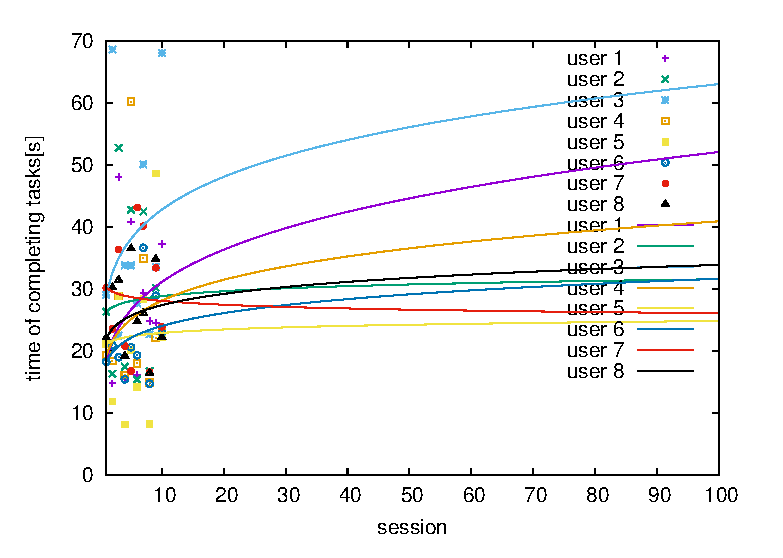
\includegraphics[width=12cm,height=8cm]{touchteika.eps} \hspace{-80pt}
	\vspace{50pt}
	\caption{タッチ操作で行った場合のタスク完了時間の低下予測}
	\label{fig:f28}
\end{figure}

\begin{table}[H]
	\begin{center}
	\begin{tabular}{|c|c|} \hline
		user & $T_n$  \\ \hline \hline
		user 1 &  $18.594×n^{0.224}$ \\
		user 2 &  $26.341×n^{0.039}$ \\
		user 3 &  $29.064×n^{0.168}$ \\
		user 4 &  $19.322×n^{0.163}$ \\
		user 5 &  $21.124×n^{0.035}$ \\
		user 6 &  $18.240×n^{0.120}$ \\
		user 7 &  $30.199×n^{-0.032}$ \\
		user 8 &  $22.140×n^{0.092}$ \\ \hline
	\end{tabular}
	\caption{タスク完了時間の低下予測(タッチ操作の場合)}
	\label{table10}
	\end{center}
\end{table}
\end{comment}

本システムの場合、最初のほうはタスク完了時間の値が大きい人が多かったが、最後のほうは操作に慣れてきて全員、50秒を切っていることが表\ref{table9}からもわかった。表\ref{table11}と表\ref{table12}より全体の平均はタッチ操作のほうが早いが、後半の平均を見るとそれぞれの差はかなり縮まってきており、最後のほうは差がほとんどなくなり、人によっては本システムのほうが早いという結果になった。
%図\ref{fig:f27}より本システムのほうでは練習のべき乗則に従っている人、従っていない人がいた。べき乗則に従っていない人は
本システムのほうで中盤で時間が極端にかかった人がいた。練習しても本システムになかなか慣れなかったことや、途中で逆に慣れてきて操作がいい加減になっていること等が原因なのではないかと考えられる。また、時々目の前に正解の駅があったとしても見落としてしまうことも考えられる。図\ref{fig:f25}と図\ref{fig:f26}からタッチ操作よりも本システムのほうがセッション数を増やせば増やすほどタスク完了時間が低下する傾向の人が多いことがわかった。

\subsection{アンケート結果}
ここではアンケートの結果を示す。

\subsubsection{スクロールの精度}
なかなか本システムの操作に慣れずスクロール精度については悪いと思っている人が多かった。スクロールの精度の向上はもちろんだが、操作方法の説明、注意すべき点についてもう少し詳しく説明すべきだった。

\begin{table}[H]
	\begin{center}
	\begin{tabular}{|c|c|c|c|c|} \hline
		1.とても良い & 2.良い & 3.普通 & 4.悪い & 5.とても悪い \\ \hline \hline
		0人 & 1人 & 1人 & 5人 & 1人  \\ \hline
	\end{tabular}
	\caption{スクロールの精度はどうでしたか?}
	\label{table2}
	\end{center}
\end{table}

\subsubsection{ズームの精度}
スクロールに比べるとズームの精度はまだ良いと思っている人が多かったようだった。良いと答えた1人はズームに関してはタッチ操作と違って指が邪魔にならなくて良いと感じたようだった。

\begin{table}[H]
	\begin{center}
	\begin{tabular}{|c|c|c|c|c|} \hline
		1.とても良い & 2.良い & 3.普通 & 4.悪い & 5.とても悪い \\ \hline \hline
		0人 & 1人 & 3人 & 4人 & 0人  \\ \hline
	\end{tabular}
	\caption{ズームの精度はどうでしたか?}
	\label{table3}
	\end{center}
\end{table}

\subsubsection{疲労感の有無}
疲労感に関しては個人差が見られた。本システムに慣れた人は疲労感をほとんど感じなかったようだが、なかなか慣れなくて操作がうまくいかなかった人は疲労感を少し感じたようだった。

\begin{table}[H]
	\begin{center}
	\begin{tabular}{|c|c|c|c|c|} \hline
		1.全くない & 2.あまりない & 3.普通 & 4.少しあった & 5.かなりあった \\ \hline \hline
		2人 & 0人 & 2人 & 4人 & 0人  \\ \hline
	\end{tabular}
	\caption{疲労感はありましたか?}
	\label{table4}
	\end{center}
\end{table}

\subsubsection{スクロールやズームをしている際の画面全体の把握のしやすさ(タッチの場合)}
全員普段からスマートフォンを使用していてタッチ操作に慣れているので特に気にならない人も多かったように見えた。

\begin{table}[H]
	\begin{center}
	\begin{tabular}{|c|c|c|c|c|} \hline
		1.とても把握しやすい & 2.把握しやすい & 3.普通 & 4.把握しづらい & 5.とても把握しづらい \\ \hline \hline
		1人 & 1人 & 5人 & 1人 & 0人  \\ \hline
	\end{tabular}
	\caption{タッチ操作の場合、スクロールやズームをしている際に画面全体を把握しやすかったですか?}
	\label{table5}
	\end{center}
\end{table}

\subsubsection{スクロールやズームをしている際の画面全体の把握のしやすさ(FingCVの場合)}
本研究の目的である画面領域を最大限生かすという点はこの設問より改善されていると思った人が多かったことがわかった。しかし、3人はそう思わなかったことがわかった。理由はカメラのプレビュー画面に集中しすぎてしまうことが原因で画面全体が逆に見えなくなってしまうからではないかと考えられる。

\begin{table}[H]
	\begin{center}
	\begin{tabular}{|c|c|c|c|c|} \hline
		1.とても把握しやすい & 2.把握しやすい & 3.普通 & 4.把握しづらい & 5.とても把握しづらい \\ \hline \hline
		2人 & 3人 & 0人 & 3人 & 0人  \\ \hline
	\end{tabular}
	\caption{本システムの場合、スクロールやズームをしている際に画面全体を把握しやすかったですか?}
	\label{table6}
	\end{center}
\end{table}

\subsubsection{タッチ操作とFingCVの比較}
全員タッチ操作に慣れていたので本システムに関して違和感を感じた人が多かった。もう少しスクロールやズームの精度を向上できれば評価は違っただろう。

\begin{table}[H]
	\begin{center}
	\begin{tabular}{|c|c|c|c|c|} \hline
		1.とても良い & 2.良い & 3.同じくらい & 4.悪い & 5.とても悪い \\ \hline \hline
		0人 & 0人 & 0人 & 8人 & 0人  \\ \hline
	\end{tabular}
	\caption{タッチ操作と比べて本システムはどうでしたか?}
	\label{table7}
	\end{center}
\end{table}

\subsubsection{総合的なFingCVの評価}
違和感を感じた人がほとんどだったが1人は本システムを良いと感じたようである。ゲームや地図アプリを使用している際に指が邪魔になるので本システムは使えるのではないかと思ったようである。

\begin{table}[H]
	\begin{center}
	\begin{tabular}{|c|c|c|c|c|} \hline
		1.とても良い & 2.良い & 3.普通 & 4.悪い & 5.とても悪い \\ \hline \hline
		0人 & 1人 & 4人 & 3人 & 0人  \\ \hline
	\end{tabular}
	\caption{総合的に見て本システムはどうでしたか?}
	\label{table8}
	\end{center}
\end{table}

\subsubsection{追加してほしい機能}

\begin{itemize}
	\item タップ(6人)
	\item 進む、戻る(2人)
	\item スクロールとズームに切り替えるのを無くしてほしい
	\item スクロール時とズーム時の切り替え(画面のタッチ)位置を工夫してほしい
	\item ズーム位置を指定できるようにしてほしい
	\item タブ一覧の表示
\end{itemize}

\subsubsection{その他}

\begin{itemize}
	\item カメラのプレビュー画面に集中しすぎてしまう(3人)
	\item スクロールが逆のほうが良かった(2人)
	\item モード切替時のフィードバックが欲しい(2人)
	\item スクロール幅を指の振り幅と合わせて欲しい。ズームも同様(2人)
	\item スクロールをするときに手の形や位置に気を付けなければならないのが少し面倒に感じた
	\item スクロールがちゃんと認識されない時があった
	\item ズームは使いやすい。できれば上下ではなく左右がいい
	\item 端を長押ししている間画面が動くのは個人的に好き
	\item カメラが横についていると手が楽な気がした
	\item スマホのスクロール方法と似ていたので直感的に操作できた
	\item 本システムではタッチ操作と比べて指で隠れずに画面が見れた
	\item ゲームや地図アプリで使ってみたい
	\item 左手の長押しする場所が途中でわからなくなった
	\item もっと他にもズームやスクロールの操作を行える実験をやってみたい
	\item 全体的なレスポンス(地図の表示)が悪いのでそれを直さないと語りづらい
	\item もっとスペックの高い端末使おう
	\item 精度をもっと上げてほしい
	\item 位置センサとの併用を考えてほしい
	\item どこを長押しすればいいのか明確にしてほしい
	\item 指を反対向きにするとタッチ操作と同じになる
	\item タッチ操作も最初は慣れるまで時間がかかったので、この操作も慣れることで使いやすさが変わっていくと思う
	\item 指先が円の中(デフォルト位置)に戻ったことを知らせてほしい
	\item カメラと指を近づけないと操作しにくいということに気づくまではまともに操作出来なかった。そこに気づくと操作しやすい
\end{itemize}

\subsection{おわりに}
本章では実験結果、アンケート結果について述べ、これらの結果についての考察を述べた。次章は本論文のまとめを述べ、今回の研究の改善すべき点や今後の展望について詳しく述べる。

\newpage
\section{おわりに}
\subsection{まとめ}
最初の章では研究背景としてスマートフォンの画面の表示領域を最大限に生かすような研究が行われてきたことを述べ、それらの問題点を解決するために本研究では端末の内蔵カメラを用いて画面の表示領域を狭める事なく、スマートフォンを操作する手法を提案、実装、評価することを本研究の目的として述べた。

第2章では関連研究として背面から端末を操作をする研究と内臓カメラを用いて操作する研究の特徴や問題点について述べた。

第3章では本システムであるFingCVの概要として仕様や操作方法を説明した。その後、スワイプ操作、ピンチイン、ピンチアウト操作、閲覧履歴の移動操作の3つの操作モードについて詳しく説明をした。

第4章ではまずFingCVの実装環境について述べ、その後に指認識について肌色領域の抽出の方法、手の検出の方法、指先の検出の方法について詳しく述べた。その次にブラウザの操作処理について、操作モードの切替方法、指先のジェスチャ検出の方法について詳しく説明をした。

第5章ではFingCVについての評価実験の説明をした。まず、実験目的や被験者情報について述べた後、実際に行った実験内容について説明をし、最後にアンケートの内容について述べた。

第6章では実験の結果と考察について述べた。最初に、練習のべき乗則について詳しく説明をし、実験の測定結果をFingCVの方法とタッチ操作の方法についてグラフで表示した。FingCVのほうがセッション数を増やせば増やすほどタスク完了時間が低下することが実験結果からわかった。その次にアンケートの結果について述べた。なかなか操作に慣れない人も多く、スクロールやズームの精度がそこまで良くなかったため、FingCVの総合的な評価としてはあまり良くなかった。個人差もかなりあったように見られた。画面の表示領域を最大限生かすという点は改善されたという意見が多かったことがわかった。しかし、カメラのプレビュー画面に集中しすぎて画面全体が見づらくなってしまうという問題点も挙がった。

\subsection{改善すべき点}
実験結果よりスクロールやズームの精度があまり良くなかったことがわかったため、指認識についてもう少し改める必要があると感じた。画像処理を使って実装しているため背景の色や照明に気を付けなければならないこともあったので、誤認識を減らすような処理がもっと必要であると痛感した。

ブラウザの操作処理についてもスクロールやズームの幅をもう少し自由に設定できるようにすべきだったと感じた。操作モードの切替時のフィードバックについてもあったほうがわかりやすいと思った。また、スクロールの方向をタッチ操作と同様にしたが、逆のほうが良いという意見もあったので両方の方法でできるように実装すべきだった。

\subsection{展望}
改善すべき点も多かったが、内蔵カメラだけでスマートフォンの操作をするのは困難な場面も多く、限界を感じた。アンケートの結果でもあったが、位置センサ等の独自のハードウェアを付けたほうがより安定した処理ができ、もっと快適に操作ができるようになり、タッチ操作の方法と同等以上のシステムが作成できるのではないかと考えた。また、スマートフォンの処理能力は年々上がっているので、より新しい端末を使うことでもっと安定した操作が期待できるだろう。

\section*{謝辞}
ご指導を頂いた赤池先生、角田先生並びに、実験の被験者やその他の面でも日々ご助力を頂いた研究室の皆様方に厚くお礼を申し上げます。

\newpage
\begin{thebibliography}{数字}
  \bibitem{wigdor} Daniel Wigdor, Clifton Forlines, Patrick Baudisch, John Brnwell, Chia Shen: LucidTouch:A See-through Mobile Device, UIST’07 Proceedings of the 20th annual ACM on symposium on User interface software and technology, p.269-278 (2007)
  \bibitem{kobayashi} 小林 茂, 鈴木 宣也, 赤羽 亨, 蛭田 直, 近藤 崇司, 伊豆 裕一, 米山 貴久, 横内 恭人: 裏タッチインターフェース 画面の背面から操作するインターフェースの提案, インタラクション論文集2010, SA24 (2010)
  \bibitem{takeda1} 竹田 智, 岩田 満:内蔵カメラを用いたスマートフォン操作手法の提案, 平成24年度電子情報通信学会東京支部学生会研究発表会論文集, p.205 (2013)
  \bibitem{takeda2} 竹田 智, 岩田 満: 内蔵カメラを用いたジェスチャによるスマートフォン操作手法の検討, 情報処理学会第76回全国大会論文集, 4-25,26 (2014)
  \bibitem{okada} 岡田浩臣, 星野孝総: HMDを用いた仮想ガジェットの開発, ViEWビジョン技術の実利用ワークショップ講演論文集2012, ROMBUNNO.IS2-D3(2012)
  \bibitem{subway} Subway Map Visualization jQuery Plugin, <http://kalyani.com/2010/10/subway-map-visualization-jquery-plugin/>
  \bibitem{rosenzu} canvasを使って地下鉄の路線図を描けるjQueryプラグインで東京の地下鉄の路線図を描いてみた, <http://webdrawer.net/javascript/subwaycanvas.html>
\end{thebibliography}

\newpage
\section*{付録 本実験アンケート}
本実験後に回答してもらった各被験者のアンケート用紙を添付する。

\end{document}